\begin{figure}[h!]
    \centering
    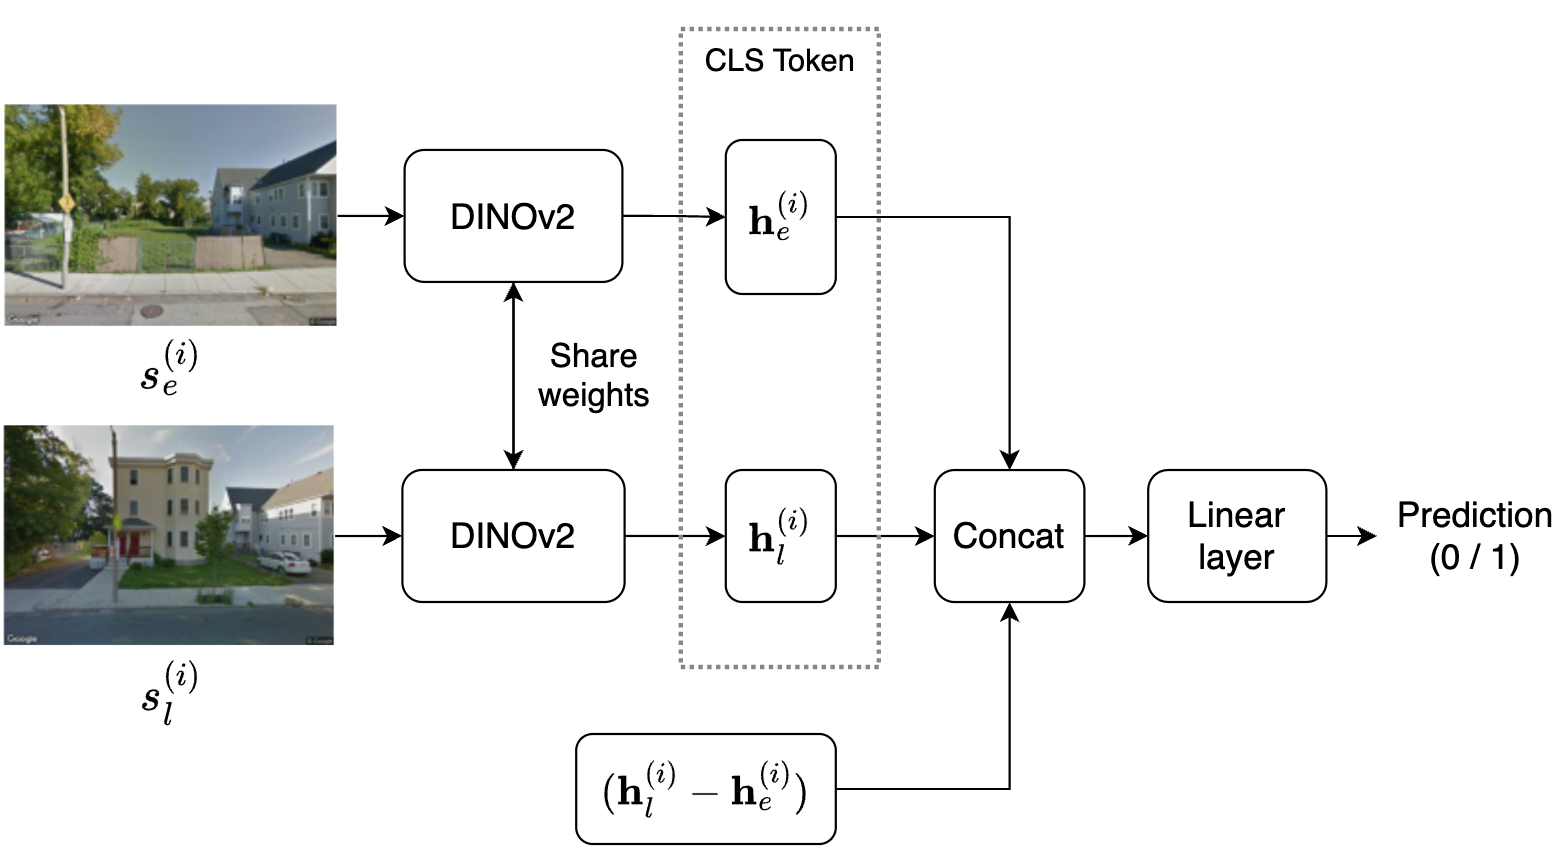
\includegraphics[width=1.05\linewidth]{figure/change_model.png}
    \caption{Overview of the change detection model architecture. Pairs of input images are processed using Siamese-based networks with DINOv2 as the backbone. The CLS tokens serve as the image representation, with a subsequent linear layer projecting them to a prediction score.}
    \label{fig:change_model}
\end{figure}


% \begin{figure}[h!]
%     \centering
%     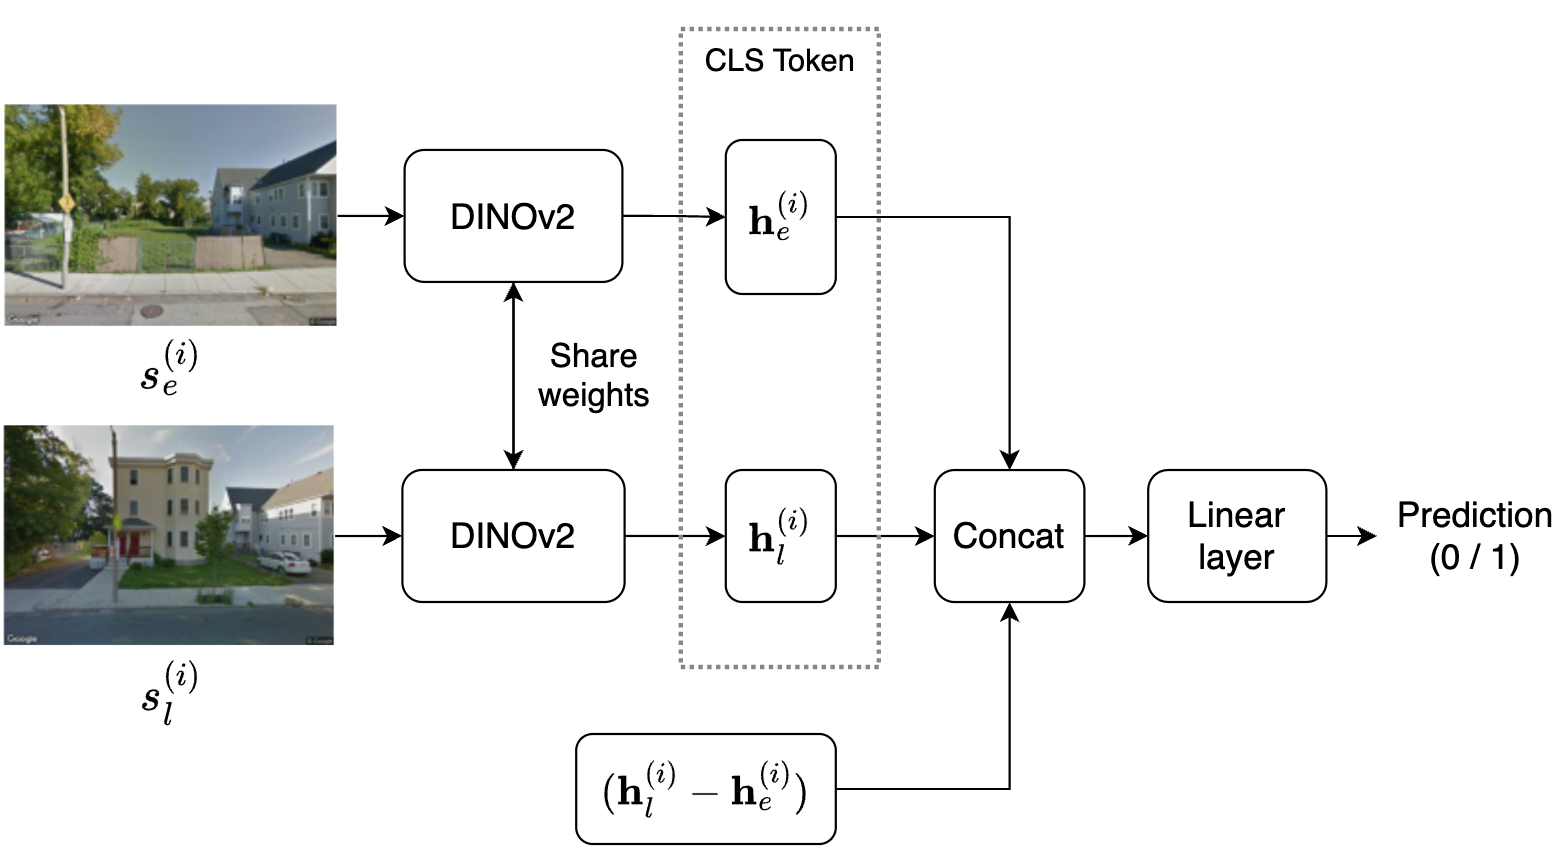
\includegraphics[width=1.05\linewidth]{figure/change_model.png}
%     \caption{Overview of the change detection model architecture. Each pair of input images are passed through a Siamese-based networks with DINOv2 as backbone modules, we treat the CLS token as the representation of each image and add a linear layer to preject into a prediction score.}
%     \label{fig:change_model}
% \end{figure}